
\section{Programme scientifique et technique, organisation du projet / Scientific and technical programme, Project organisation}
\begin{xcomment}  
A titre indicatif : de 5 à 10  pages pour ce chapitre, en fonction du nombre de tâches
\end{xcomment}

\subsection{Programme scientifique et structuration du projet  / Scientific programme, project structure}
\begin{xcomment}  
 Pr\'esentez le programme scientifique et justifiez la d\'ecomposition en tâches du programme de travail en coh\'erence avec les objectifs poursuivis. 
Utilisez un diagramme pour pr\'esenter les liens entre les diff\'erentes tâches (organigramme technique)
Les tâches repr\'esentent les grandes phases du projet. Elles sont en nombre limit\'e.
Le cas \'ech\'eant (programmes exigeant la pluridisciplinarit\'e), d\'emontrer l'articulation entre les disciplines scientifiques.
N'oubliez pas les tâches correspondant à la diss\'emination et à la valorisation, à d\'ecrire en d\'etails au §4.

\end{xcomment}

The DADA project includes fundamental research in multiple disciplines, focusing on a single object of study - the virtual actor. Work will be divided into four main work packages: (1) procedural animation of isolated actors; (2) procedural animation of interaction between actors; (3) authoring and real-time control; (4) user evaluations. 


\begin{xcomment}  
thierry : ce passage là doit probablement etre remonté au dessus pour l'explication générale du flux entre WPs. 
\end{xcomment}



WP1 focuses on animation models for isolated actors.  The inputs that are used by the methods to be developed in this work package are procedural animation scenario as output by WP2.  Such a scenario includes in particular detailed indications on the action to be realized (walk from one point to another, carry object, knock on door, throw object, lift object, move object), the mood of the character (neutral, happy, afraid, angry, anxious, sad, proud, shameful) and a set of static information about the character that change the way people move (age, gender, morphology, corpulence, expressivity level, etc). Both action and mood may vary with time among the animation while static information remain fixed per nature.  These three sets of information will be refered hereafter as \textit{action context}, \textit{mood context} and \textit{profile context}. . 

WP2 focuses on animation models for groups of actors. Based on the dramatic score composed by the director, patterns of actions and reactions of the virtual actors will be computed, 
taking into account the social relations between their characters, and the physical constraints imposed by the stage. This work package will be responsible for synchronising the behaviours
and the movements of the virtual actors between cues given by the director.  This work package will compute only a small number of degrees of freedom of the virtual actors, and provide the spatial and temporal context in which the full body animation is computed in details.

WP3 focuses on the control of the virtual actors by the director. Research work will be conducted to define a consistent and expressive  language that the director can use to 
compose the dramatic score for the actors. Novel authoring tools will be designed and developed to support the language with intuitive and efficient graphical user interfaces. 
This work package will also be responsible for executing  the animations produced by WP1 and WP2 in real-time using state-of-the-art game technologies present in the Unity 5 
game engine. 

WP4 focuses on the user evaluation of the proposed technologies from the perspective of a theatre director. Exercises for one to three actors will be developed to test 
the capabilities of the system. Example scenes of theatre plays will be chosen and staged for virtual actors. The usability of the system and the quality of the animation
will be evaluated with a number of real-life scenarios, including virtual rehearsals for real-life productions, production of theatre performances for virtual worlds and
teaching of theatre techniques.

\begin{figure}[htbp]
\begin{center}
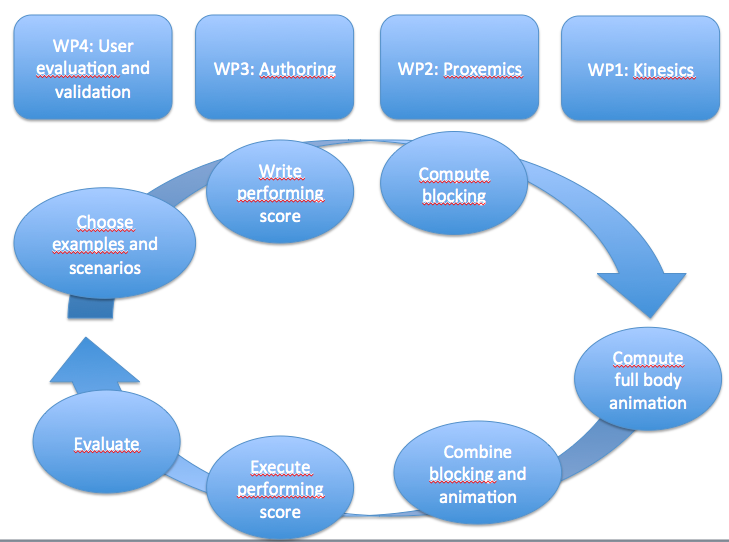
\includegraphics[width=0.9\linewidth]{DADAWORKFLOW.png}
\caption{Data flow between work packages: Through the authoring tool (WP3), a script is elaborated by a theater director (WP4); it gives direction to group of virtual
actors which act out autonomously the commands of the script to position toward each other and in the virtual space (WP2). The behaviors of each actor is computed 
taking into account their emotional states and social relations (WP1).}
\label{default}
\end{center}
\end{figure}


\endinput